\documentclass{lug}

\usepackage{fontawesome}
\usepackage{etoolbox}
\usepackage{etoolbox}
\usepackage{textcomp}
\usepackage[nodisplayskipstretch]{setspace}
\usepackage{xspace}

\AtBeginEnvironment{minted}{\singlespacing\fontsize{10}{10}\selectfont}

\makeatletter
\patchcmd{\beamer@sectionintoc}{\vskip1.5em}{\vskip0.5em}{}{}
\makeatother

\newcommand{\pmidg}[1]{\parbox{\widthof{#1}}{#1}}
\newcommand{\splitslide}[4]{
    \noindent
    \begin{minipage}{#1 \textwidth - #2 }
        #3
    \end{minipage}%
    \hspace{ \dimexpr #2 * 2 \relax }%
    \begin{minipage}{\textwidth - #1 \textwidth - #2 }
        #4
    \end{minipage}
}

\title{Filesystems}
\author{Sumner Evans and Sam Sartor}
\institute{Mines Linux Users Group}

\begin{document}

\section{Introduction}

\begin{frame}{What are Filesystems?}
    \begin{itemize}
        \item Filesystems manage the storage and retrieval of files from storage
            media.
        \item Filesystems are an abstraction layer between storage media (SSDs,
            HDDs, disk drives, even tape drives).
        \item Filesystems exist on \textit{partitions}, physically contiguous
            segments of the disk.
    \end{itemize}
\end{frame}

\begin{frame}{Filesystems are Responsible for\ldots}
    \begin{itemize}
        \item \textbf{Space management:} filesystems allocate and manage space
            in discrete chunks. Filesystems must keep track of what data is
            stored at each chunk.
        \item \textbf{Filenames:} identify a storage location in the file
            system. Can be case sensitive (ext4) or case insensitive (HFS,
            NTFS).
        \item \textbf{Directories (folders):} group files into separate
            collections. Modern filesystems allow arbitrary nesting of
            directories.
        \item \textbf{Metadata:} filesystems store book-keeping information
            about their contents (e.g. file sizes, last accessed date, owner and
            permissions, etc.).
        \item \textbf{Access Control:} prevent unauthorized access to files on
            disk.
        \item \textbf{Data Integrity:} filesystems must be resilient to failure,
            some are better at this than others.
    \end{itemize}
\end{frame}

\section{History of Filesystems}
\begin{frame}{The First Filesystems}
    \splitslide{0.60}{1em}{
    The filesystem was originally thought of as part of the operating system.

    One of the first filesystems that had a name was DECTape. DECTape stored an
    astoundingly small 184 kilobytes (kilo, not mega) of data per tape on the
    PDP-8.
    }{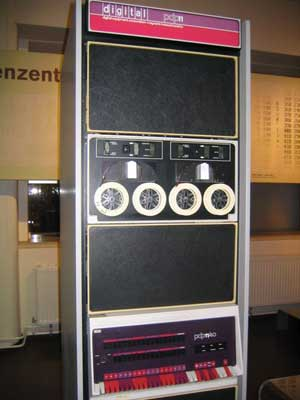
\includegraphics[width=0.4\textheight]{./graphics/dectape.jpg}}
\end{frame}

\section{Current Filesystems}

\section{Linux}
\begin{frame}{ex4}
\end{frame}

\section{Windows \& mac}
\begin{frame}{NTFS}
\end{frame}

\begin{frame}{HFS, HFS+ \& APFS}
\end{frame}

\section{Flashdrives}
\begin{frame}{FAT32}
\end{frame}

\begin{frame}{Other Options}
\end{frame}

\section{Alternative Filesystems}
\begin{frame}{Btrfs}
\end{frame}

\begin{frame}{XFS}
\end{frame}

\begin{frame}{ZFS}
\end{frame}

\begin{frame}{TFS}
\end{frame}

\section{Network Filesystems}
\begin{frame}{What is a network filesystem?}
\begin{center}
    You can access remote storage devices over the internet using a
    \emph{network filesystem}.
\end{center}
\end{frame}

\begin{frame}{NFS}
\end{frame}

\begin{frame}{Samba}
\end{frame}

\section{Virtual Filesystems}
\begin{frame}{What is a virtual filesystem?}
\begin{center}
    There is no reason why a filesystem needs to be backed by a real partition
    on a real storage device. The exist plenty of \emph{virtual filesystems}
    that are purely procedural or abstract other kinds of devices.
\end{center}
\end{frame}

\begin{frame}{tmpfs}
\end{frame}

\begin{frame}{proc filesystem}
\end{frame}

\begin{frame}{FUSE}
\begin{itemize}
    \item Filesystem in Userspace (FUSE) is an interface for creating
    filesystems without writing any kernel-level code
    \item Available in Linux, FreeBSD, OpenBSD, NetBSD, OpenSolaris, Minix 3,
    Android, and macOS
    \item Access through libfuse for C (bindings exist for Python, Rust, etc.)
\end{itemize}
\end{frame}

\begin{frame}{sshfs}
\begin{itemize}
    \item Implemented using FUSE
    \item Mount a directory on a remote system through SSH
\end{itemize}
\end{frame}

\section{Configuration/maintenance}

\begin{frame}{\ldots}
\end{frame}

\begin{frame}[standout]
    \Huge
    Questions?
\end{frame}

\begin{frame}{References}
    \begin{itemize}
        \item \url{https://en.wikipedia.org/wiki/File_system}
        \item \url{http://www.tldp.org/LDP/sag/html/filesystems.html}
        \item \url{https://arstechnica.com/gadgets/2008/03/past-present-future-file-systems/2/}
    \end{itemize}
\end{frame}

\end{document}
